\chapter{Diagramme des fonctionnalités}

Le diagramme des fonctionnalités permet de mettre en perspective les fonctionnalités du projet entre elles. Les fonctionnalités, les intrants et les extrants du produit y sont représentés, ainsi que leurs relations. En effet, certaines fonctionnalités sont reliés entre elles, et certaines sont reliés aux entrées et aux sorties du système.

\begin{figure}[h]
  \centering
  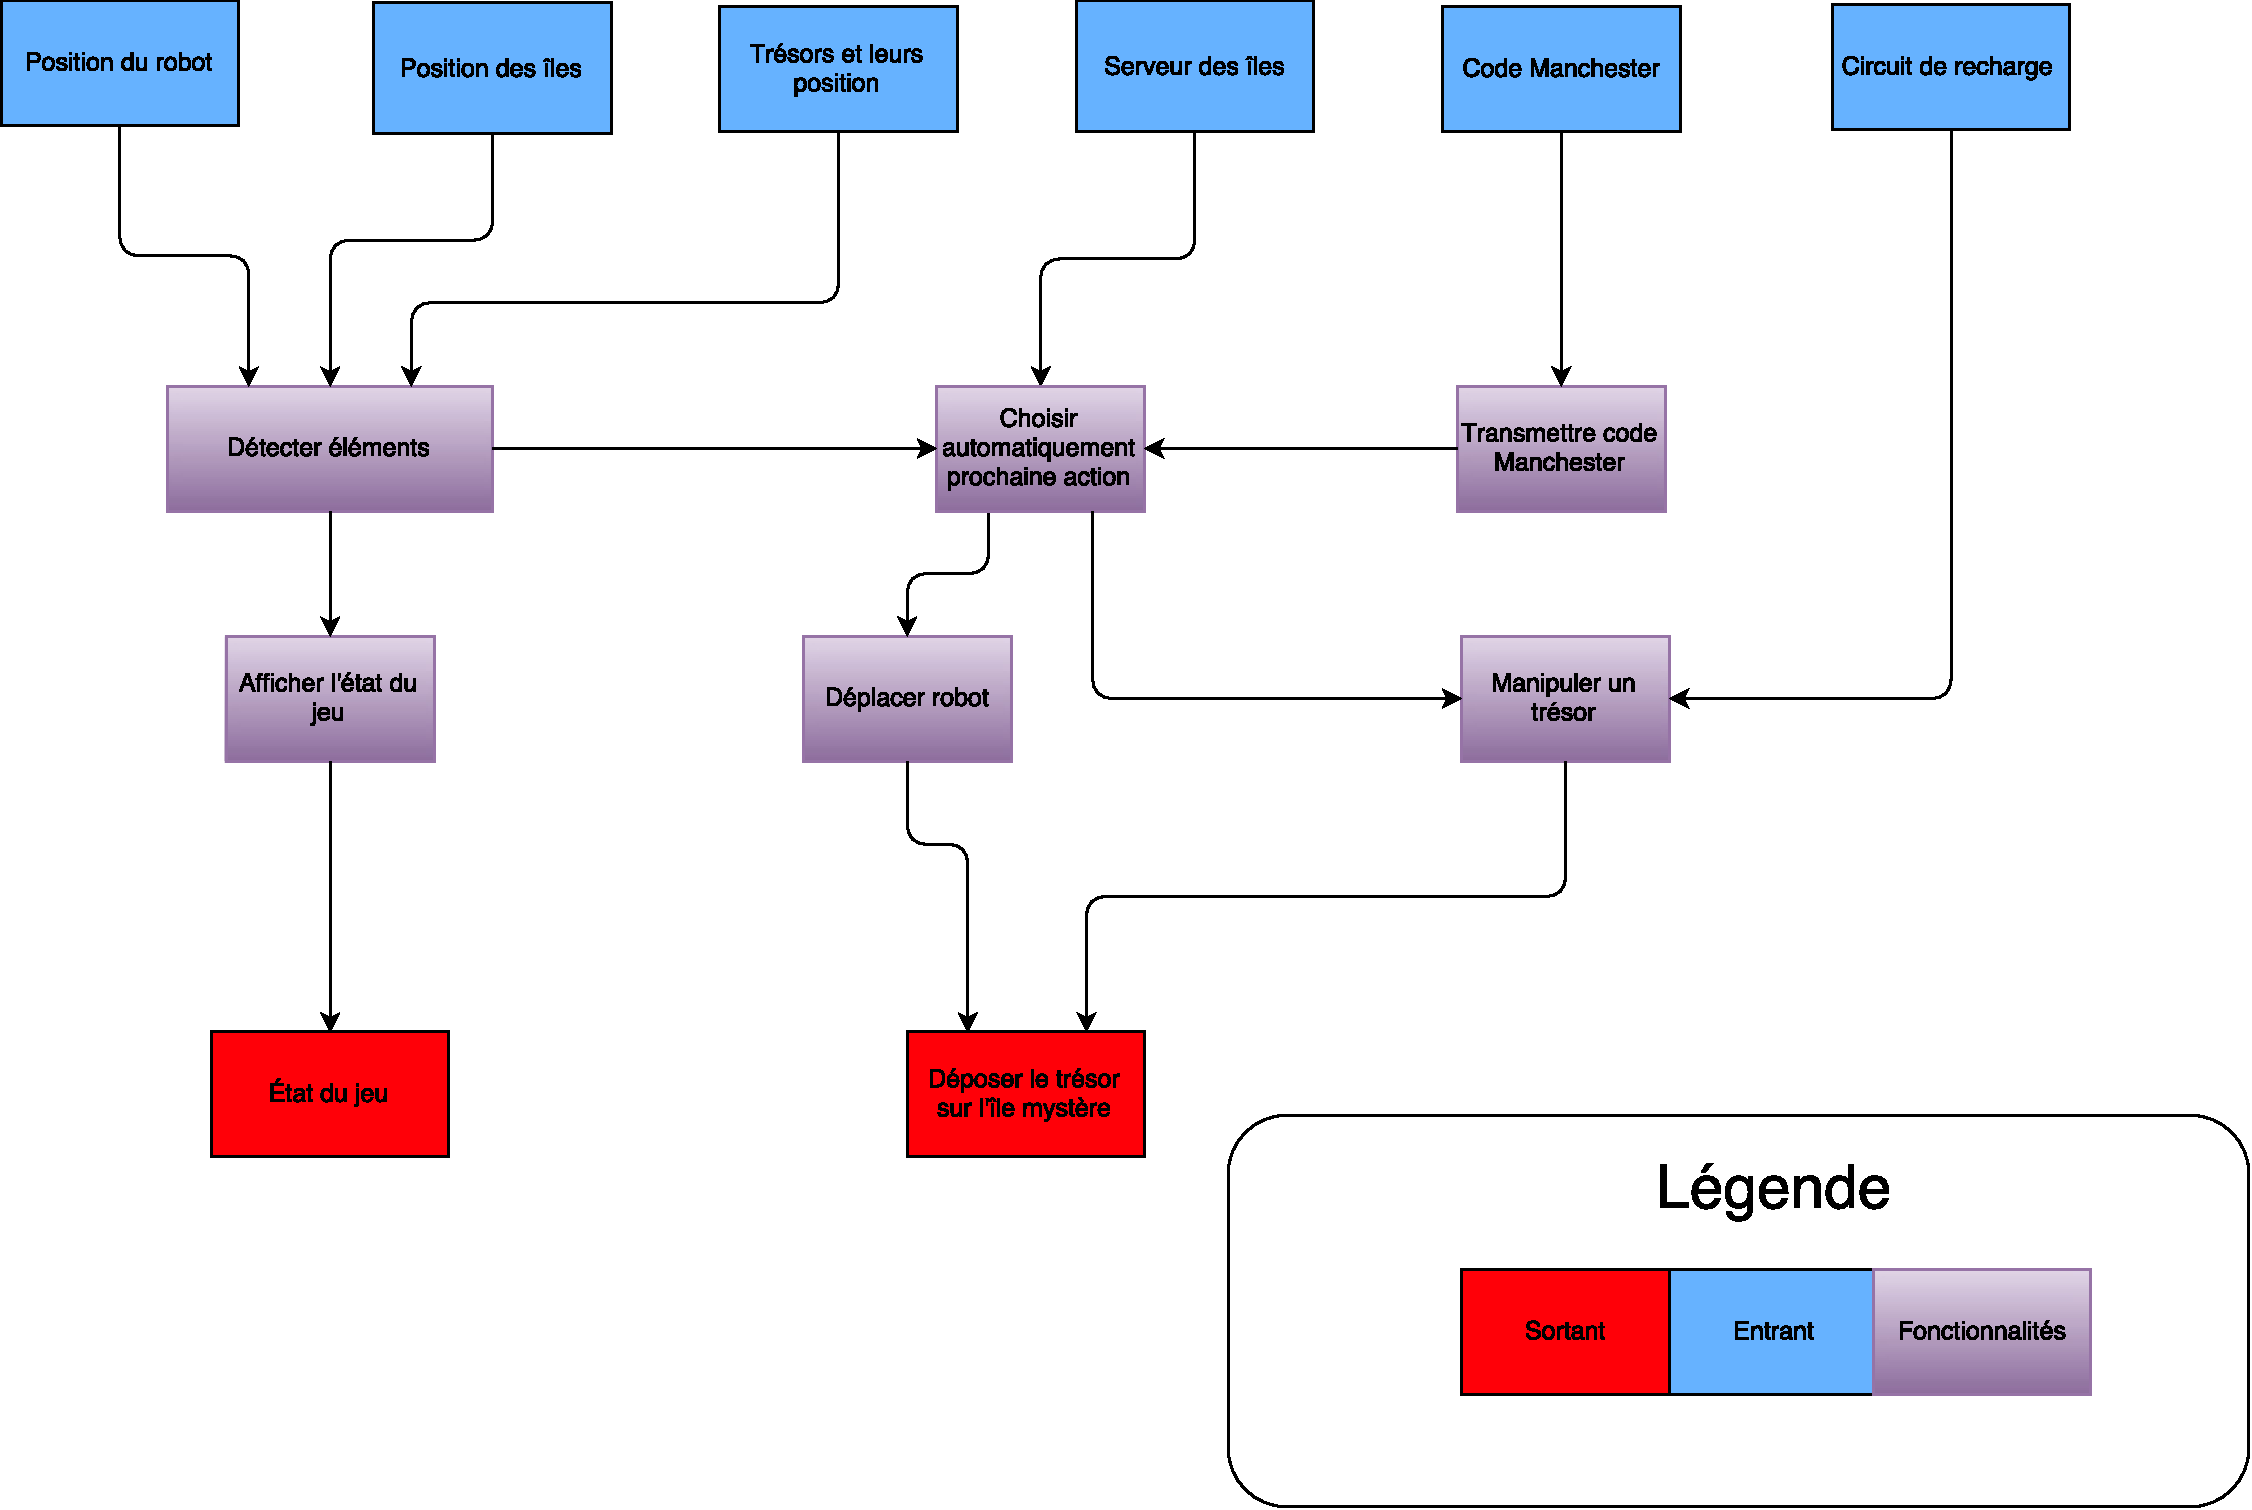
\includegraphics[scale=0.4]{resources/diag_fonc.pdf}
  \caption{Diagramme fonctionnel}
\end{figure}
